% !TEX root = thesis.tex

\section{Discussion}
\label{sec:disc}


\subsection{Discussion}
\begin{figure}[htb]
\centering
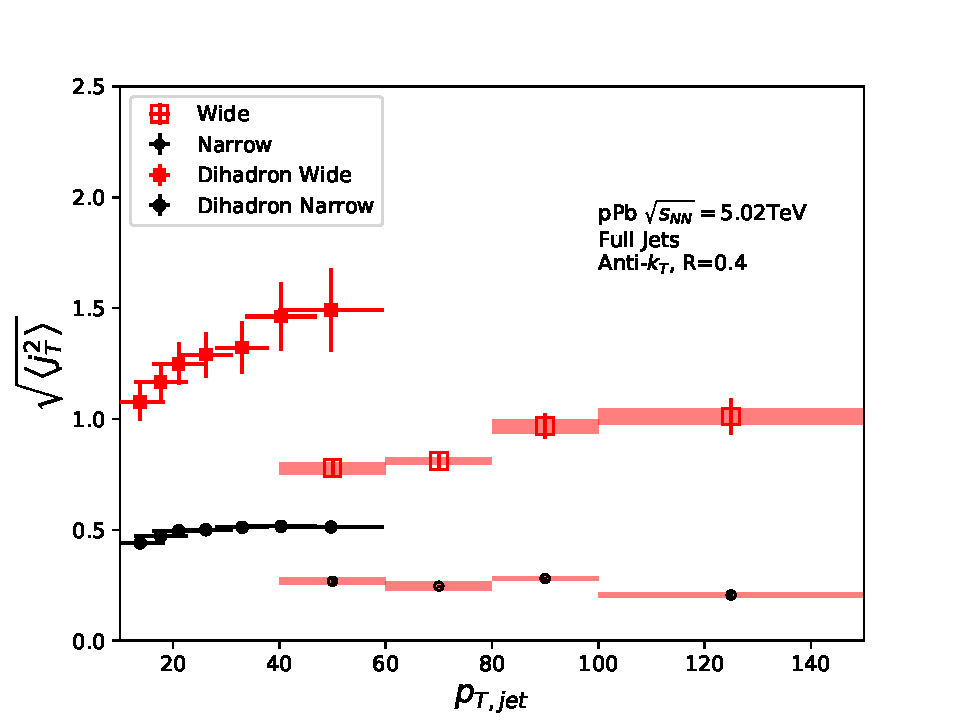
\includegraphics[width=0.55\textwidth]{figures/results/RMSWithSystematics_DihadronJetPt}
%\subfigure{ 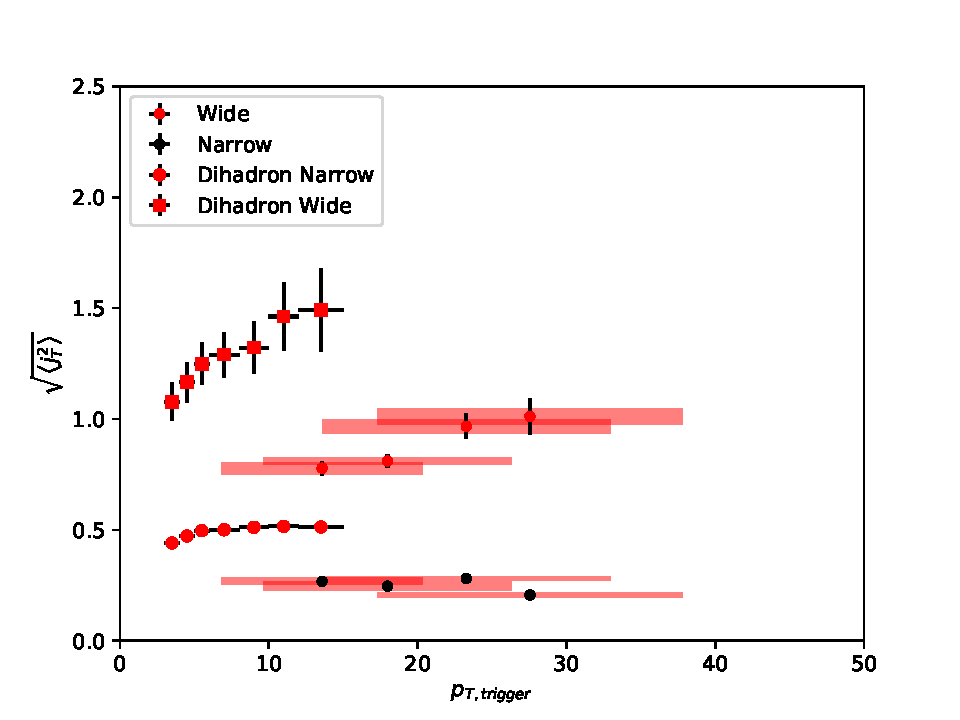
\includegraphics[width = 0.42\textwidth]{figures/results/RMSWithSystematics_DihadronTriggerPt}}
%\subfigure{ 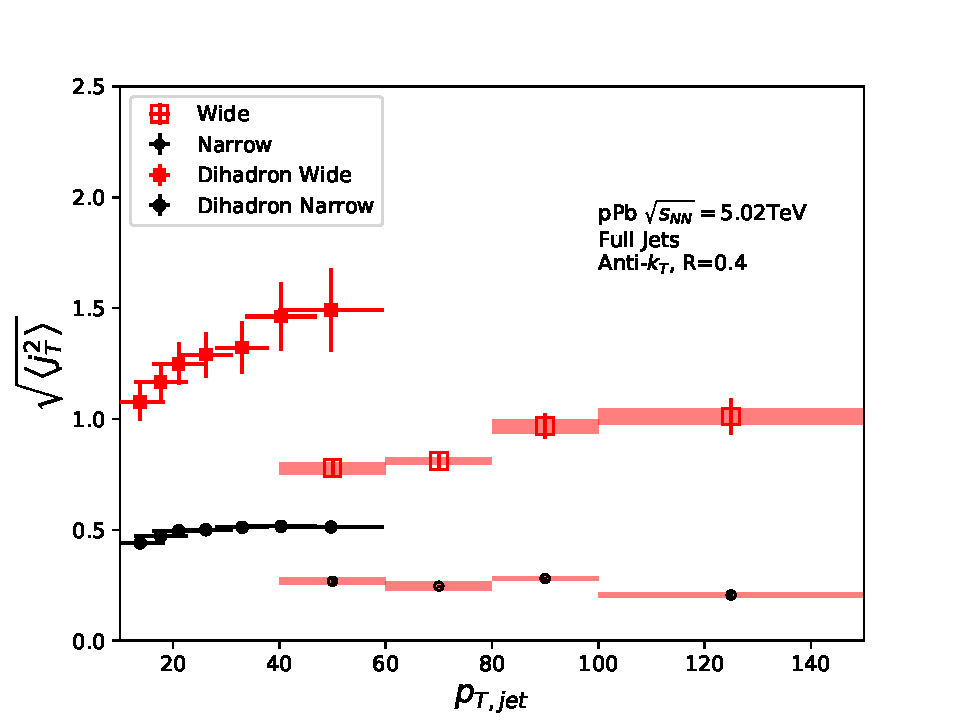
\includegraphics[width = 0.42\textwidth]{figures/results/RMSWithSystematics_DihadronJetPt}}
\caption{Comparison of results with dihadron $\jt{}$ results. Dihadron trigger $\pt{}$ bins are converted to jet $\pt{}$  bins  using observed mean  $\pt{jet}$ values in $\pt{trigger}$ bins. Dihadron results are for $0.2 < x_{||} < 0.4$ }
\label{fig:DihadronComparison}
\end{figure}

Comparison to $\jt{}$ results from dihadron analysis ~\cite{ALICEjt} is shown in Fig. \ref{fig:DihadronComparison}. Trigger $\pt{}$ bins used in dihadron analysis are converted to jet $\pt{}$ bins using observed average jet $\pt{}$ values in leading track momentum bins. Simlarly jet $\pt{}$ bins are converted to $\pt{trigger}$ bins using average leading track $\pt{}$ values in $\pt{jet}$ bins.

The trends are similar in dihadron and jet $\jt{}$ results. Wide component RMS values tend to increase with increasing $\pt{trigger}$/$\pt{jet}$. Narrow component RMS increases slightly in dihadron analysis but not in jet $\jt{}$, WHY? (Depends on $x_{||}$ bin in dihadron)

In general dihadron $\jt{}$ gives wider distributions with larger RMS values. In jet analysis the cone size limits width and thus the RMS values. With increasing cone size one gets increasing wide RMS values as seen in Fig. \ref{fig:Rcomparison}. This should be the dominant factor.

\begin{figure}[htp]
\centering
\begin{subfigure}{0.49\textwidth}
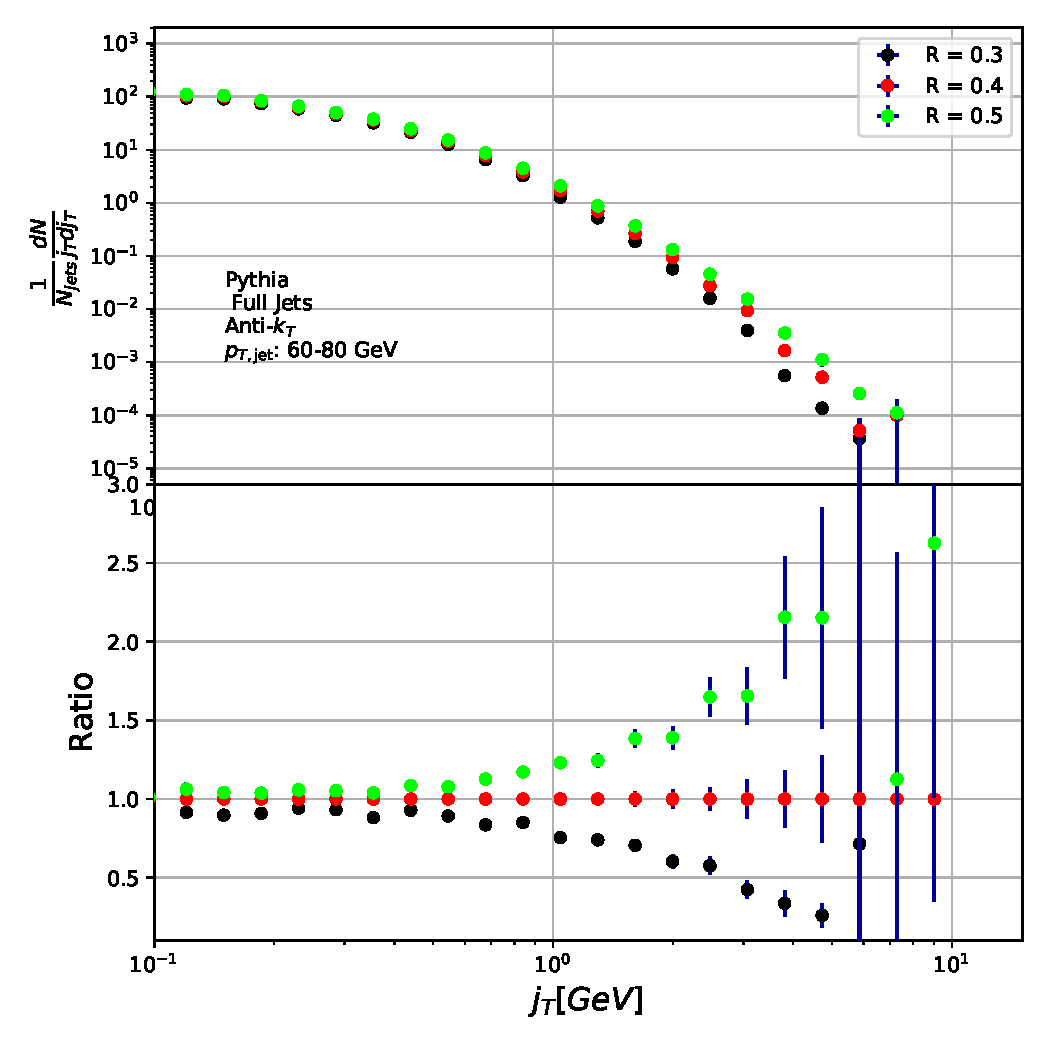
\includegraphics[width = 0.4\textwidth]{figures/results/RcomparisonSignalPt6080.pdf}
\end{subfigure}
\begin{subfigure}{0.49\textwidth}
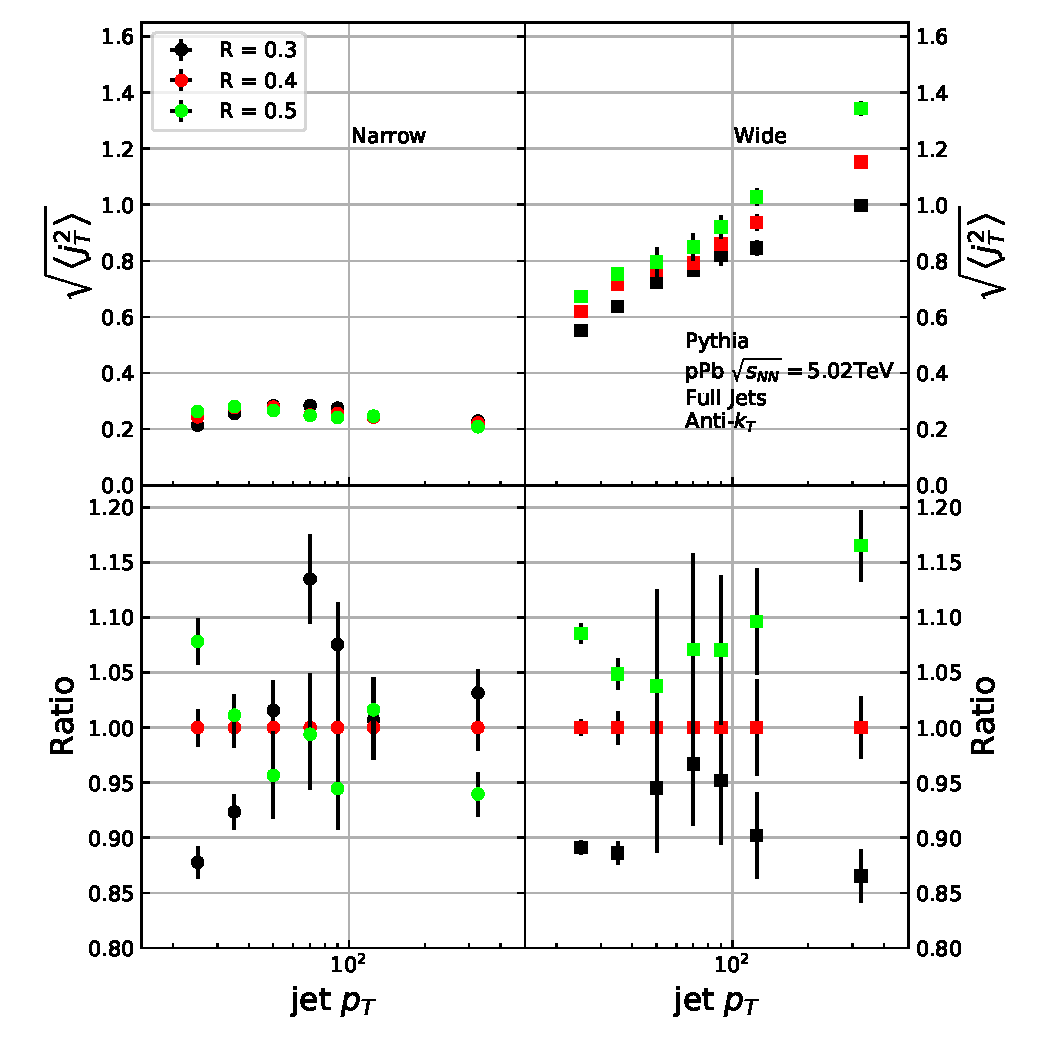
\includegraphics[width = 0.4\textwidth]{figures/results/RcomparisonRMS.pdf}
\end{subfigure}
\caption[\textsc{Pythia} $R$ parameters $\jt{}$]{Effect of changing $R$ parameter in jet finding on $\jt{}$ distributions}
\label{fig:Rcomparison}
\end{figure}


Effect of the $R$ parameter choice is studied in \textsc{Pythia}. Having a fixed cone puts hard limits on the possible $\jt{}$ values. Increasing the cone size loosens these limits and allows higher $\jt{}$ values. The results are shown in Fig. \ref{fig:Rcomparison}. Left hand side shows the $\jt{}$ distributions. There is very little change in low $\jt{}$ but at high $\jt{}$ the yield increases. 

This is also seen in the RMS values shown in the right hand side of Fig. \ref{fig:Rcomparison}, where the change in wide component RMS is about 10\% when going from $R=0.4$ to $R=0.3$ or $R=0.5$. With the narrow component values the situation is less clear. At low jet $\pt{}$ larger $R$ parameter leads to larger RMS values, but at hight $\pt{jet}$ the situation is reversed; increasing the $R$ parameter decreases RMS values.

Additionally the leading track is an imperfect estimate of the jet/original parton. Because the leading track in general is at an angle compared to the jet axis, the resulting $\jt{}$ values are different. In practice the jet axis found by the jet finding algrorithm tends to minimize the average $\jt{}$ of jet constituents. Thus the yield at high $\jt{}$ is limited and the RMS values are smaller.

A \textsc{Pythia} study was performed where $\jt{}$ was calculated with respect to the leading track momentum, instead of the jet axis. The results are shown in Fig. \ref{fig:RefComparison}. The resulting $\jt{}$ distributions are significantly wider than $\jt{}$ distributions from the typical method. The effect seems to be larger than the effect seen in comparing different $R$ values.

\begin{figure}[htp]
\centering
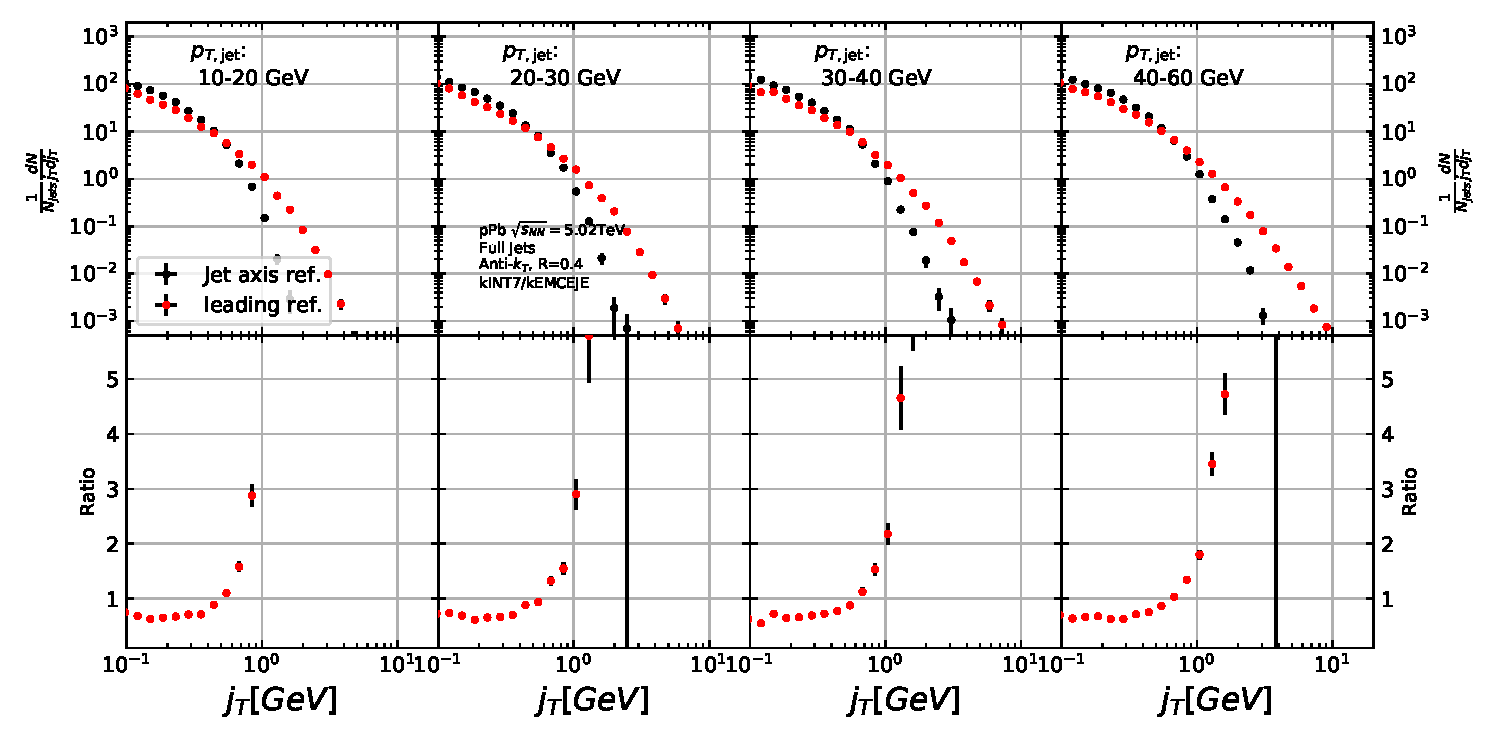
\includegraphics[width=0.55\textwidth]{figures/results/JetVsLeadingRefConst.pdf}
\caption{Results of calculating $\jt{}$ with respect to the jet axis or the leading hadron. The assumption is that because the leading hadron is an imperfect estimate of the jet axis, low $\jt{}$ tracks should on average be shifted to higher $\jt{}$}
\label{fig:RefComparison}
\end{figure}


\pagebreak
\FloatBarrier
\section{Summary}
\label{sec:sum}
In this work two distinct $\jt{}$ components were extracted for narrow and wide contributions using jet reconstruction. RMS values for both components were obtained. The width of the wide component is found to increase for increasing $\pt{jet}$. This is in part explained by the changing kinematical limits when going to higher $\pt{jet}$ which allows higher $\pt{track}$. Additionally the larger phase space allows stronger parton splitting. The results are qualitatively compatible with previous studies that studied $\jt{}$ using two-particle correlations.

